% Options for packages loaded elsewhere
\PassOptionsToPackage{unicode}{hyperref}
\PassOptionsToPackage{hyphens}{url}
%
\documentclass[
  a4paper,
]{book}

\usepackage{amsmath,amssymb}
\usepackage{lmodern}
\usepackage{iftex}
\ifPDFTeX
  \usepackage[T1]{fontenc}
  \usepackage[utf8]{inputenc}
  \usepackage{textcomp} % provide euro and other symbols
\else % if luatex or xetex
  \usepackage{unicode-math}
  \defaultfontfeatures{Scale=MatchLowercase}
  \defaultfontfeatures[\rmfamily]{Ligatures=TeX,Scale=1}
\fi
% Use upquote if available, for straight quotes in verbatim environments
\IfFileExists{upquote.sty}{\usepackage{upquote}}{}
\IfFileExists{microtype.sty}{% use microtype if available
  \usepackage[]{microtype}
  \UseMicrotypeSet[protrusion]{basicmath} % disable protrusion for tt fonts
}{}
\makeatletter
\@ifundefined{KOMAClassName}{% if non-KOMA class
  \IfFileExists{parskip.sty}{%
    \usepackage{parskip}
  }{% else
    \setlength{\parindent}{0pt}
    \setlength{\parskip}{6pt plus 2pt minus 1pt}}
}{% if KOMA class
  \KOMAoptions{parskip=half}}
\makeatother
\usepackage{xcolor}
\usepackage[top=2.5cm,,bottom=2.5cm,,left=2cm,,right=2cm]{geometry}
\setlength{\emergencystretch}{3em} % prevent overfull lines
\setcounter{secnumdepth}{5}
% Make \paragraph and \subparagraph free-standing
\ifx\paragraph\undefined\else
  \let\oldparagraph\paragraph
  \renewcommand{\paragraph}[1]{\oldparagraph{#1}\mbox{}}
\fi
\ifx\subparagraph\undefined\else
  \let\oldsubparagraph\subparagraph
  \renewcommand{\subparagraph}[1]{\oldsubparagraph{#1}\mbox{}}
\fi

\usepackage{color}
\usepackage{fancyvrb}
\newcommand{\VerbBar}{|}
\newcommand{\VERB}{\Verb[commandchars=\\\{\}]}
\DefineVerbatimEnvironment{Highlighting}{Verbatim}{commandchars=\\\{\}}
% Add ',fontsize=\small' for more characters per line
\usepackage{framed}
\definecolor{shadecolor}{RGB}{241,243,245}
\newenvironment{Shaded}{\begin{snugshade}}{\end{snugshade}}
\newcommand{\AlertTok}[1]{\textcolor[rgb]{0.68,0.00,0.00}{#1}}
\newcommand{\AnnotationTok}[1]{\textcolor[rgb]{0.37,0.37,0.37}{#1}}
\newcommand{\AttributeTok}[1]{\textcolor[rgb]{0.40,0.45,0.13}{#1}}
\newcommand{\BaseNTok}[1]{\textcolor[rgb]{0.68,0.00,0.00}{#1}}
\newcommand{\BuiltInTok}[1]{\textcolor[rgb]{0.00,0.23,0.31}{#1}}
\newcommand{\CharTok}[1]{\textcolor[rgb]{0.13,0.47,0.30}{#1}}
\newcommand{\CommentTok}[1]{\textcolor[rgb]{0.37,0.37,0.37}{#1}}
\newcommand{\CommentVarTok}[1]{\textcolor[rgb]{0.37,0.37,0.37}{\textit{#1}}}
\newcommand{\ConstantTok}[1]{\textcolor[rgb]{0.56,0.35,0.01}{#1}}
\newcommand{\ControlFlowTok}[1]{\textcolor[rgb]{0.00,0.23,0.31}{#1}}
\newcommand{\DataTypeTok}[1]{\textcolor[rgb]{0.68,0.00,0.00}{#1}}
\newcommand{\DecValTok}[1]{\textcolor[rgb]{0.68,0.00,0.00}{#1}}
\newcommand{\DocumentationTok}[1]{\textcolor[rgb]{0.37,0.37,0.37}{\textit{#1}}}
\newcommand{\ErrorTok}[1]{\textcolor[rgb]{0.68,0.00,0.00}{#1}}
\newcommand{\ExtensionTok}[1]{\textcolor[rgb]{0.00,0.23,0.31}{#1}}
\newcommand{\FloatTok}[1]{\textcolor[rgb]{0.68,0.00,0.00}{#1}}
\newcommand{\FunctionTok}[1]{\textcolor[rgb]{0.28,0.35,0.67}{#1}}
\newcommand{\ImportTok}[1]{\textcolor[rgb]{0.00,0.46,0.62}{#1}}
\newcommand{\InformationTok}[1]{\textcolor[rgb]{0.37,0.37,0.37}{#1}}
\newcommand{\KeywordTok}[1]{\textcolor[rgb]{0.00,0.23,0.31}{#1}}
\newcommand{\NormalTok}[1]{\textcolor[rgb]{0.00,0.23,0.31}{#1}}
\newcommand{\OperatorTok}[1]{\textcolor[rgb]{0.37,0.37,0.37}{#1}}
\newcommand{\OtherTok}[1]{\textcolor[rgb]{0.00,0.23,0.31}{#1}}
\newcommand{\PreprocessorTok}[1]{\textcolor[rgb]{0.68,0.00,0.00}{#1}}
\newcommand{\RegionMarkerTok}[1]{\textcolor[rgb]{0.00,0.23,0.31}{#1}}
\newcommand{\SpecialCharTok}[1]{\textcolor[rgb]{0.37,0.37,0.37}{#1}}
\newcommand{\SpecialStringTok}[1]{\textcolor[rgb]{0.13,0.47,0.30}{#1}}
\newcommand{\StringTok}[1]{\textcolor[rgb]{0.13,0.47,0.30}{#1}}
\newcommand{\VariableTok}[1]{\textcolor[rgb]{0.07,0.07,0.07}{#1}}
\newcommand{\VerbatimStringTok}[1]{\textcolor[rgb]{0.13,0.47,0.30}{#1}}
\newcommand{\WarningTok}[1]{\textcolor[rgb]{0.37,0.37,0.37}{\textit{#1}}}

\providecommand{\tightlist}{%
  \setlength{\itemsep}{0pt}\setlength{\parskip}{0pt}}\usepackage{longtable,booktabs,array}
\usepackage{calc} % for calculating minipage widths
% Correct order of tables after \paragraph or \subparagraph
\usepackage{etoolbox}
\makeatletter
\patchcmd\longtable{\par}{\if@noskipsec\mbox{}\fi\par}{}{}
\makeatother
% Allow footnotes in longtable head/foot
\IfFileExists{footnotehyper.sty}{\usepackage{footnotehyper}}{\usepackage{footnote}}
\makesavenoteenv{longtable}
\usepackage{graphicx}
\makeatletter
\def\maxwidth{\ifdim\Gin@nat@width>\linewidth\linewidth\else\Gin@nat@width\fi}
\def\maxheight{\ifdim\Gin@nat@height>\textheight\textheight\else\Gin@nat@height\fi}
\makeatother
% Scale images if necessary, so that they will not overflow the page
% margins by default, and it is still possible to overwrite the defaults
% using explicit options in \includegraphics[width, height, ...]{}
\setkeys{Gin}{width=\maxwidth,height=\maxheight,keepaspectratio}
% Set default figure placement to htbp
\makeatletter
\def\fps@figure{htbp}
\makeatother
\newlength{\cslhangindent}
\setlength{\cslhangindent}{1.5em}
\newlength{\csllabelwidth}
\setlength{\csllabelwidth}{3em}
\newlength{\cslentryspacingunit} % times entry-spacing
\setlength{\cslentryspacingunit}{\parskip}
\newenvironment{CSLReferences}[2] % #1 hanging-ident, #2 entry spacing
 {% don't indent paragraphs
  \setlength{\parindent}{0pt}
  % turn on hanging indent if param 1 is 1
  \ifodd #1
  \let\oldpar\par
  \def\par{\hangindent=\cslhangindent\oldpar}
  \fi
  % set entry spacing
  \setlength{\parskip}{#2\cslentryspacingunit}
 }%
 {}
\usepackage{calc}
\newcommand{\CSLBlock}[1]{#1\hfill\break}
\newcommand{\CSLLeftMargin}[1]{\parbox[t]{\csllabelwidth}{#1}}
\newcommand{\CSLRightInline}[1]{\parbox[t]{\linewidth - \csllabelwidth}{#1}\break}
\newcommand{\CSLIndent}[1]{\hspace{\cslhangindent}#1}

% \usepackage{booktabs}

\usepackage{fontspec}
%\usepackage{amsfonts}
\usepackage{amsthm}

%\usepackage{nicefrac} %好看的分數 專門放在指數  \nicefrac{1}{2}

\usepackage{amssymb}
% \allowdisplaybreaks[1]

%\usepackage{nath}
%\delimgrowth=1

\numberwithin{equation}{section}

\renewcommand{\baselinestretch}{1.2}  %字間的行距


\usepackage{xeCJK}
\setCJKmainfont{標楷體}
\XeTeXlinebreaklocale "zh"
\XeTeXlinebreakskip = 0pt plus 1pt
\defaultCJKfontfeatures{AutoFakeBold=6,AutoFakeSlant=.4}
%\usepackage{lipsum}
%\usepackage[most]{tcolorbox}

%\setlength{\leftmargini}{6pt}

%\newenvironment{tbox}{\begin{tcolorbox}[colback=white,enhanced jigsaw,breakable, boxrule = 0.2mm, ,left=6pt,right=6pt,top=1pt,bottom=1pt,arc = 0mm]}{\end{tcolorbox}}

%%%%%%%%%%%%%%%%%%%%%%%%%%%%%%%%%%%%%%%%%%%%%%%%%%%%%%%%%%%%


\newlength{\zhind}
\settowidth{\zhind}{fives}
\AtBeginDocument{\setlength{\parindent}{\zhind}}  %每行留白距離

\AtBeginDocument{\setlength{\abovedisplayskip}{10pt}}
\AtBeginDocument{\setlength{\belowdisplayskip}{10pt}}

\AtBeginDocument{\setlength{\parskip}{.6em}}  %換段落的距離

%%%%%%%%%%%%%%%%%%%%%%%%%%%%%%%%%%%%%%%%%%%%%%%%%%%%%%%%%%%%




%%%%%%%%%%%%%%%%%%%%%%%%%%%%%%%%%%%%%%%%%%%%%%%%%%%%%%%%%%%%%%%
%%%%% 課本形式的頁碼 在左右上角 
% read https://bookdown.org/yihui/rmarkdown-cookbook/latex-header.html
\usepackage{fancyhdr}   
% \fancypagestyle{plain}{%
% \fancyhf{}
% \fancyhead[L]{\leftmark}
\fancyhead[RE]{\nouppercase{\leftmark}}
\fancyhead[LO]{\nouppercase{\rightmark}}
\fancyhead[RO,LE]{\thepage}
\fancyfoot{}
% }
\renewcommand{\headrulewidth}{0pt}% Default \headrulewidth is 0.4pt



%%%%% 論文形式的頁碼 
% \usepackage{fancyhdr}
% \pagestyle{fancy}
% % center of header
% %\fancyhead[CO,CE]{Your Document Header}
% \fancyhead{}

% % center of footer
% %\fancyfoot[CO,CE]{\thepage}
% \cfoot{\thepage}

% % page number on the left of even pages and right of odd pages
% %\fancyfoot[LE,RO]{\thepage}

% \thispagestyle{fancy}

% \renewcommand{\headrulewidth}{0pt}% Default \headrulewidth is 0.4pt

%%%%%%%%%%%%%%%%%%%%%%%%%%%%%%%%%%%%%%%%%%%%%%%%%%%%%%%%%%%%%%%


%%%%%%%%%%%%%%%%%%%%%%%%
\delimitershortfall -0.1em  % 調整\left \right nested的大小
\let\originalleft\left
\let\originalright\right
\renewcommand{\left}{\mathopen{}\mathclose\bgroup\originalleft}
\renewcommand{\right}{\aftergroup\egroup\originalright}





%\usepackage{makeidx}
%\makeindex
\usepackage{imakeidx}
%\usepackage[nonewpage]{imakeidx}
%\indexsetup{level=\section*,toclevel=section,headers={Stellenregister}{\indexname}}%
%\indexsetup{level=\section*,toclevel=section,noclearpage}
\makeindex[name=term,title={Index of Terms}]
\makeindex[name=notation,title={Index of Notations}]

\usepackage[nottoc]{tocbibind}

%\usepackage[index]{kantlipsum}




% 要放在 \usepackage{imakeidx} 後面 
\makeindex


% 顯示 label !
\usepackage[left]{showlabels}
\renewcommand{\showlabelfont}{\ttfamily\tiny}


%\usepackage{mathtools} % 只列出有 eqref 的equation num  在 tinytex 會出錯
%\mathtoolsset{showonlyrefs=true}
%\mathtoolsset{showonlyrefs,showmanualtags}

%% 更改水平線長度  % footnote 會GG
%\let\oldrule=\rule
%\renewcommand{\rule}[1]{\oldrule{\linewidth}}

\usepackage{url}  % bib url 用的



%% cols

\newenvironment{columns}[1][]{}{}

\newenvironment{column}[1]{\begin{minipage}{#1}\ignorespaces}{%
\end{minipage}
\ifhmode\unskip\fi
\aftergroup\useignorespacesandallpars}

\def\useignorespacesandallpars#1\ignorespaces\fi{%
#1\fi\ignorespacesandallpars}

\makeatletter
\def\ignorespacesandallpars{%
  \@ifnextchar\par
    {\expandafter\ignorespacesandallpars\@gobble}%
    {}%
}
\makeatother



% 聖經
% \usepackage[left]{lineno}
% \linenumbers



% 圖片強制位置
\usepackage{float}

% subfig
%\usepackage{subfig}
% \usepackage[margin=10pt]{subfig}
%\setlength{\subfigcapmargin}{5pt}
%\captionsetup[subfigure]{width=0.9\textwidth}

% 動畫
% \usepackage{animate}


% Do not page break for Environment
% 這樣弄的話 環境裡面不能放圖片
\AtBeginEnvironment{theorem}{\bigskip\begin{center}\begin{minipage}{\textwidth}}
\AtEndEnvironment{theorem}{\end{minipage}\end{center}\bigskip}
\AtBeginEnvironment{proposition}{\bigskip\begin{center}\begin{minipage}{\textwidth}}
\AtEndEnvironment{proposition}{\end{minipage}\end{center}\bigskip}
\AtBeginEnvironment{lemma}{\bigskip\begin{center}\begin{minipage}{\textwidth}}
\AtEndEnvironment{lemma}{\end{minipage}\end{center}\bigskip}
\AtBeginEnvironment{definition}{\bigskip\begin{center}\begin{minipage}{\textwidth}}
\AtEndEnvironment{definition}{\end{minipage}\end{center}\bigskip}
\AtBeginEnvironment{conjecture}{\bigskip\begin{center}\begin{minipage}{\textwidth}}
\AtEndEnvironment{conjecture}{\end{minipage}\end{center}\bigskip}


% pdfpages
\usepackage{pdfpages}


% \usepackage[style=authoryear,backend=biber]{biblatex}
\makeatletter
\makeatother
\makeatletter
\@ifpackageloaded{bookmark}{}{\usepackage{bookmark}}
\makeatother
\makeatletter
\@ifpackageloaded{caption}{}{\usepackage{caption}}
\AtBeginDocument{%
\ifdefined\contentsname
  \renewcommand*\contentsname{Table of contents}
\else
  \newcommand\contentsname{Table of contents}
\fi
\ifdefined\listfigurename
  \renewcommand*\listfigurename{List of Figures}
\else
  \newcommand\listfigurename{List of Figures}
\fi
\ifdefined\listtablename
  \renewcommand*\listtablename{List of Tables}
\else
  \newcommand\listtablename{List of Tables}
\fi
\ifdefined\figurename
  \renewcommand*\figurename{Figure}
\else
  \newcommand\figurename{Figure}
\fi
\ifdefined\tablename
  \renewcommand*\tablename{Table}
\else
  \newcommand\tablename{Table}
\fi
}
\@ifpackageloaded{float}{}{\usepackage{float}}
\floatstyle{ruled}
\@ifundefined{c@chapter}{\newfloat{codelisting}{h}{lop}}{\newfloat{codelisting}{h}{lop}[chapter]}
\floatname{codelisting}{Listing}
\newcommand*\listoflistings{\listof{codelisting}{List of Listings}}
\usepackage{amsthm}
\theoremstyle{plain}
\newtheorem{proposition}{Proposition}[chapter]
\theoremstyle{remark}
\renewcommand*{\proofname}{Proof}
\newtheorem*{remark}{Remark}
\newtheorem*{solution}{Solution}
\makeatother
\makeatletter
\@ifpackageloaded{caption}{}{\usepackage{caption}}
\@ifpackageloaded{subcaption}{}{\usepackage{subcaption}}
\makeatother
\makeatletter
\@ifpackageloaded{tcolorbox}{}{\usepackage[many]{tcolorbox}}
\makeatother
\makeatletter
\@ifundefined{shadecolor}{\definecolor{shadecolor}{rgb}{.97, .97, .97}}
\makeatother
\makeatletter
\makeatother
\ifLuaTeX
  \usepackage{selnolig}  % disable illegal ligatures
\fi
\IfFileExists{bookmark.sty}{\usepackage{bookmark}}{\usepackage{hyperref}}
\IfFileExists{xurl.sty}{\usepackage{xurl}}{} % add URL line breaks if available
\urlstyle{same} % disable monospaced font for URLs
\hypersetup{
  pdftitle={DL-Note},
  pdfauthor={ChoCho},
  hidelinks,
  pdfcreator={LaTeX via pandoc}}

\title{DL-Note}
\author{ChoCho}
\date{11/7/22}

\begin{document}
\frontmatter
\maketitle
\ifdefined\Shaded\renewenvironment{Shaded}{\begin{tcolorbox}[boxrule=0pt, frame hidden, borderline west={3pt}{0pt}{shadecolor}, sharp corners, breakable, interior hidden, enhanced]}{\end{tcolorbox}}\fi

\renewcommand*\contentsname{Table of contents}
{
\setcounter{tocdepth}{2}
\tableofcontents
}
\mainmatter
\bookmarksetup{startatroot}

\hypertarget{preface}{%
\chapter*{Preface}\label{preface}}
\addcontentsline{toc}{chapter}{Preface}

\markboth{Preface}{Preface}

asdasdasdasdsada das dasd asd

Iam in altera philosophiae parte. quae est quaerendi ac disserendi, quae
logikh dicitur, iste vester plane, ut mihi quidem videtur, inermis ac
nudus est. tollit definitiones, nihil de dividendo ac partiendo docet,
non quo modo efficiatur concludaturque ratio tradit, non qua via
captiosa solvantur ambigua distinguantur ostendit; iudicia rerum in
sensibus ponit, quibus si semel aliquid falsi pro vero probatum sit,
sublatum esse omne iudicium veri et falsi putat. Confirmat autem illud
vel maxime, quod ipsa natura, ut ait ille, sciscat et probet, id est
voluptatem et dolorem. ad haec et quae sequamur et quae fugiamus refert
omnia. quod quamquam Aristippi est a Cyrenaicisque melius liberiusque
defenditur, tamen eius modi esse iudico, ut nihil homine videatur
indignius. ad maiora enim quaedam nos natura genuit et conformavit, ut
mihi quidem videtur. ac fieri potest, ut errem, sed ita prorsus
existimo, neque eum Torquatum, qui hoc primus cognomen invenerit, aut
torquem illum hosti detraxisse, ut aliquam ex eo perciperet corpore
voluptatem, aut cum Latinis tertio consulatu conflixisse apud Veserim
propter voluptatem; quod vero securi percussit filium, privavisse se
etiam videtur multis voluptatibus, cum ipsi naturae patrioque amori
praetulerit ius maiestatis atque imperii. quid? T. Torquatus, is qui
consul cum Cn. Octavio fuit, cum illam severitatem in eo filio adhibuit,
quem in adoptionem D. Silano emancipaverat, ut eum Macedonum legatis
accusantibus, quod pecunias praetorem in provincia cepisse arguerent,
causam apud se dicere iuberet reque ex utraque parte audita pronuntiaret
eum non talem videri fuisse in imperio, quales eius maiores fuissent, et
in conspectum suum venire vetuit, numquid tibi videtur de voluptatibus
suis cogitavisse? Sed ut omittam pericula, labores, dolorem etiam, quem
optimus quisque pro patria et pro suis suscipit, ut non modo nullam
captet, sed etiam praetereat omnes voluptates, dolores denique quosvis
suscipere malit quam deserere ullam officii partem, ad ea, quae hoc non
minus declarant, sed videntur leviora, veniamus. Quid tibi, Torquate,
quid huic Triario litterae, quid historiae cognitioque rerum, quid
poetarum evolutio, quid tanta tot versuum memoria voluptatis affert? nec
mihi illud dixeris: `Haec enim ipsa mihi sunt voluptati, et erant illa
Torquatis.' Numquam hoc ita defendit Epicurus neque Metrodorus aut
quisquam eorum, qui aut saperet aliquid aut ista didicisset. et quod
quaeritur saepe, cur tam multi sint Epicurei, sunt aliae quoque causae,
sed multitudinem haec maxime allicit, quod ita putant dici ab illo,
recta et honesta quae sint, ea facere ipsa per se laetitiam, id est
voluptatem. homines optimi non intellegunt totam rationem everti, si ita
res se habeat. nam si concederetur, etiamsi ad corpus nihil referatur,
ista sua sponte et per se esse iucunda, per se esset et virtus et
cognitio rerum, quod minime ille vult expetenda. Haec igitur Epicuri non
probo, inquam. De cetero vellem equidem aut ipse doctrinis fuisset
instructior - est enim, quod tibi ita videri necesse est, non satis
politus iis artibus, quas qui tenent, eruditi appellantur - aut ne
deterruisset alios a studiis. quamquam te quidem video minime esse
deterritum. Quae cum dixissem, magis ut illum provocarem quam ut ipse
loquerer, tum Triarius leniter arridens: Tu quidem, inquit, totum
Epicurum paene e philosophorum choro sustulisti. Quid ei reliquisti,
nisi te, quoquo modo loqueretur, intellegere, quid diceret? Aliena dixit
in physicis nec ea ipsa, quae tibi probarentur; si qua in iis corrigere
voluit, deteriora fecit. disserendi artem nullam habuit. voluptatem cum
summum bonum diceret, primum in eo ipso parum vidit, deinde hoc quoque
alienum; nam ante Aristippus, et ille melius. addidisti ad extremum
etiam indoctum fuisse. Fieri, inquam, Triari, nullo pacto potest, ut non
dicas, quid non probes eius, a quo dissentias. quid enim me prohiberet
Epicureum esse, si probarem, quae ille diceret? cum praesertim illa
perdiscere ludus esset. Quam ob rem dissentientium inter se
reprehensiones non sunt vituperandae, maledicta, contumeliae, tum
iracundiae, contentiones concertationesque in disputando pertinaces
indignae philosophia mihi videri solent. Tum Torquatus: Prorsus, inquit,
assentior; neque enim disputari sine reprehensione nec cum iracundia aut
pertinacia recte disputari potest. sed ad haec, nisi molestum est, habeo
quae velim. An me, inquam, nisi te audire vellem, censes haec dicturum
fuisse?

\leavevmode\vadjust pre{\hypertarget{prp-ASD}{}}%
\begin{proposition}[asdasdsad]\label{prp-ASD}

adsd sapd apsdjap dij \(f(x) = y.\)

\end{proposition}

Proposition~\ref{prp-ASD}

\hypertarget{asd}{%
\section*{ASD}\label{asd}}
\addcontentsline{toc}{section}{ASD}

\markright{ASD}

\begin{center}\rule{0.5\linewidth}{0.5pt}\end{center}

\bookmarksetup{startatroot}

\hypertarget{appendix}{%
\chapter{Appendix}\label{appendix}}

\begin{Shaded}
\begin{Highlighting}[]
\KeywordTok{class}\NormalTok{ A:}
    \KeywordTok{def} \FunctionTok{\_\_init\_\_}\NormalTok{(}\VariableTok{self}\NormalTok{):}
        \VariableTok{self}\NormalTok{.b }\OperatorTok{=} \DecValTok{1}
\end{Highlighting}
\end{Shaded}

\begin{Shaded}
\begin{Highlighting}[]
\NormalTok{A.\_\_dict\_\_}
\end{Highlighting}
\end{Shaded}

\begin{verbatim}
mappingproxy({'__module__': '__main__',
              '__init__': <function __main__.A.__init__(self)>,
              '__dict__': <attribute '__dict__' of 'A' objects>,
              '__weakref__': <attribute '__weakref__' of 'A' objects>,
              '__doc__': None})
\end{verbatim}

\begin{Shaded}
\begin{Highlighting}[]
\NormalTok{a }\OperatorTok{=}\NormalTok{ A()}
\NormalTok{a.b}
\end{Highlighting}
\end{Shaded}

\begin{verbatim}
1
\end{verbatim}

\begin{Shaded}
\begin{Highlighting}[]
\KeywordTok{def}\NormalTok{ add\_to\_class(Class):  }\CommentTok{\#@save}
    \KeywordTok{def}\NormalTok{ wrapper(obj):}
        \BuiltInTok{setattr}\NormalTok{(Class, obj.}\VariableTok{\_\_name\_\_}\NormalTok{, obj)}
    \ControlFlowTok{return}\NormalTok{ wrapper}
\end{Highlighting}
\end{Shaded}

\begin{Shaded}
\begin{Highlighting}[]
\AttributeTok{@add\_to\_class}\NormalTok{(A)}
\KeywordTok{def}\NormalTok{ do(}\VariableTok{self}\NormalTok{):}
    \BuiltInTok{print}\NormalTok{(}\StringTok{\textquotesingle{}Class attribute "b" is\textquotesingle{}}\NormalTok{, }\VariableTok{self}\NormalTok{.b)}
\end{Highlighting}
\end{Shaded}

\begin{Shaded}
\begin{Highlighting}[]
\NormalTok{A.\_\_dict\_\_}
\end{Highlighting}
\end{Shaded}

\begin{verbatim}
mappingproxy({'__module__': '__main__',
              '__init__': <function __main__.A.__init__(self)>,
              '__dict__': <attribute '__dict__' of 'A' objects>,
              '__weakref__': <attribute '__weakref__' of 'A' objects>,
              '__doc__': None,
              'do': <function __main__.do(self)>})
\end{verbatim}

\begin{center}\rule{0.5\linewidth}{0.5pt}\end{center}

\begin{Shaded}
\begin{Highlighting}[]
\ImportTok{import}\NormalTok{ torch}
\ImportTok{import}\NormalTok{ torch.nn }\ImportTok{as}\NormalTok{ nn}
\ImportTok{import}\NormalTok{ torch.optim }\ImportTok{as}\NormalTok{ optim}
\ImportTok{import}\NormalTok{ torch.utils.data }\ImportTok{as}\NormalTok{ data}
\ImportTok{import}\NormalTok{ torchvision.models }\ImportTok{as}\NormalTok{ models}
\ImportTok{import}\NormalTok{ torchvision.datasets }\ImportTok{as}\NormalTok{ dset}
\ImportTok{import}\NormalTok{ torchvision.transforms }\ImportTok{as}\NormalTok{ transforms}
\ImportTok{from}\NormalTok{ torch.autograd }\ImportTok{import}\NormalTok{ Variable}
\ImportTok{from}\NormalTok{ torchvision.models.vgg }\ImportTok{import}\NormalTok{ model\_urls}
\ImportTok{from}\NormalTok{ torchviz }\ImportTok{import}\NormalTok{ make\_dot}


\NormalTok{batch\_size }\OperatorTok{=} \DecValTok{3}
\NormalTok{learning\_rate }\OperatorTok{=}\FloatTok{0.0002}
\NormalTok{epoch }\OperatorTok{=} \DecValTok{50}
\NormalTok{resnet }\OperatorTok{=}\NormalTok{ models.resnet50(pretrained}\OperatorTok{=}\VariableTok{True}\NormalTok{)}

\NormalTok{x }\OperatorTok{=}\NormalTok{ torch.zeros(}\DecValTok{1}\NormalTok{, }\DecValTok{3}\NormalTok{, }\DecValTok{224}\NormalTok{, }\DecValTok{224}\NormalTok{, dtype}\OperatorTok{=}\NormalTok{torch.}\BuiltInTok{float}\NormalTok{, requires\_grad}\OperatorTok{=}\VariableTok{False}\NormalTok{)}
\NormalTok{out }\OperatorTok{=}\NormalTok{ resnet(x)}
\NormalTok{make\_dot(out)  }\CommentTok{\# plot graph of variable, not of a nn.Module}
\end{Highlighting}
\end{Shaded}

\begin{figure}[H]

{\centering 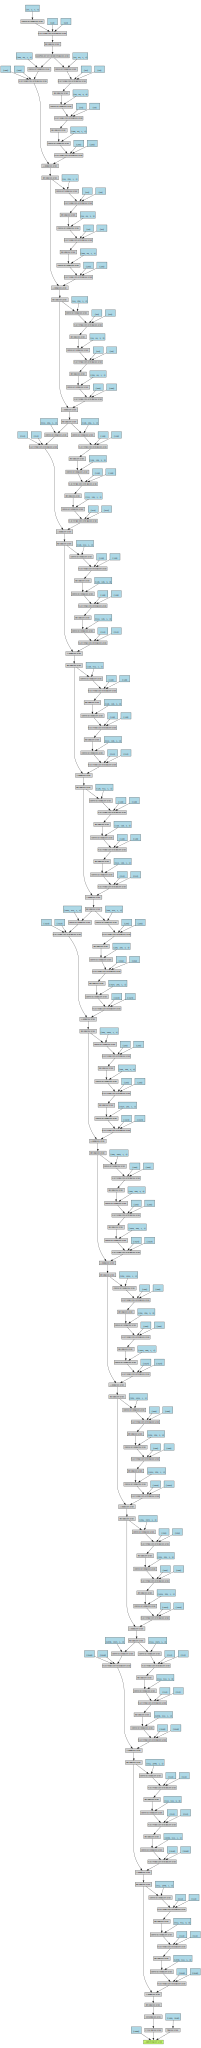
\includegraphics{./appendix_py_files/figure-pdf/cell-8-output-1.svg}

}

\end{figure}

\bookmarksetup{startatroot}

\hypertarget{references}{%
\chapter*{References}\label{references}}
\addcontentsline{toc}{chapter}{References}

\markboth{References}{References}

\hypertarget{refs}{}
\begin{CSLReferences}{0}{0}
\end{CSLReferences}


\backmatter

\end{document}
